%----------------------------------------
\chapter{\analysis}
%----------------------------------------
\section{FIT Allokáció} \label{sec:fit_allocation}
Az ipari rendszerek egyre összetettebbekké váltak az évek során. 
Emellett mostanság egyre több ilyen rendszer tartalmaz elektronikát és szoftvert, 
tehát a funkcionális biztonságnak folyamatosan nő a fontossága.\cite{Schabe}

A RAMS\footnote{Reliability, Availability, Maintainability and Safety} követelmények allokációja szerves részét képezi az alacsonyabb szinten lévő alrendszerek tervezésének rendszer mérnöki folyamatoban.
A allokáció célja, hogy megtalálja a leghatékonyabb fizikai architektúrát, ami megfelel a rendszerszintű követelményeknek és az allokáció funkcionális viselkedés analizálása által szervezett.
Amikor RAMS konstukció szükséges minden teljesítménybeli követelményfajtára - megbízhatóság, elérhetőség, karbantarthatóság, biztonságosság - külön kell az allokációs folyamatot végezni.
Az allokációs módszerek a négy különböző karakterisztikára hasonlók. \cite{en60300-3-1}

Amikor az allokáció a tervezés olyan korai fázisában kezdődik, amikor még nincs elegendő rendelkezésre álló információ az allokációt folyamatosan frissíteni kell a funkcionális analízis során.
A rendszer alacsonyabb szintjein lévő allokáció szükséges a termék meghatározási fázishoz és céljaihoz \cite{en60300-1}:
\begin{itemize}
	\item Hogy igazolja a teljes rendszer RAMS követelméyneinek megvalósíthatóságát,
	\item Hogy meghatározzon ellenőrizhető RAMS design követelményeket alacsony szinten és
	\item Hogy meghatározzon egyértelmű és megvalósítható RAMS követelményeket az alrendszerek és komponensek számára.
\end{itemize}
Általánosságban az allokációs folyamat a következő lépésekből áll:
\begin{itemize}
	\item A rendszer tanulmányozása
	\item Azon területek megtalálása, ahol a terv és a hozzá tartozó RAMS karakterisztika információk elérhetők.
	\item Alkalmas súlyok hozzárendelése és
	\item Meghatározni a magasszintű követelményhez való hozzájárulását
\end{itemize}


A safety integrity level (SIL) egy diszkrét érték ami meghatározza a használandó módszereket, technikákat a véletlenszerű és szisztematikus hibák elkerülése érdekében.
A SIL-ek koncepciója már több szabvány rendszerben ki lett fejlesztve.
Ezek között legismertebb szabványok az IEC 61508, DEF-STAN-0056, EN 50126, EN 50128, EN 50129 és még sok más.

A SIL-nek két fő aspektusa van:
\begin{enumerate}
    \item Egy cél hibaráta, amit a rendszernek nem szabad meghaladni, hogy tudja kezelni a véletlen hibákat
    \item Módszerek és technikák halmaza, amit a szisztematikus hibákat kezeli 
\end{enumerate}

Itt fontos megjegyezni, hogy szoftverben csak és kizárólag szisztematikus hibákat vesznek figyelembe és nincs megadva cél hibaráta. Ez abból adódik, hogy a szoftverben nincs véletlenszerű hiba.

\subsection{Különböző SIL-ek}
A \ref{tab:SILs} táblázat példát ad a SIL-ek és a tűrhető hibaráta kapcsolatára, ahogy három szabvány, az IEC 61508, az EN 50129 és a DEF-STAN-0056 definiálja.

A tűrhető hibaráta (THR) egy eszköz veszélyes hibáinak maximális rátája, amit a szabvány definiál bizonyos safety integrity szinthez.
Látni kell azt, hogy bár az IEC és EN szabványoknál azonosak a THR értékek, a DEF-STAN-0056-ban eltér.
Ezért a szabványok közti átjárás nem mindig triviális.
Attól még, hogy a THR értékek hasonlóak az IEC és EN szabványok között, az rendszer szintű hibaelkerülő módszerek különböznek, ezért ezek a SIL-ek sem ugyan azok.
\begin{table}[ht]
	\footnotesize
	\centering
	\begin{tabular}{ l c c }
		\toprule
		SIL & IEC 61508/EN 50129 & DEF-STAN-0056 \\
		\midrule
		1 & \(10^{-6}/h \leq\) THR \(< 10^{-5}/h\) & Frequent \(\approx 10^{-2}/h\)\\
		2 & \(10^{-7}/h \leq\) THR \(< 10^{-6}/h\)  & Probable \(\approx 10^{-4}/h\)\\
		3 & \(10^{-8}/h \leq\) THR \(< 10^{-7}/h\)  & Occasional \(\approx 10^{-6}/h\)\\
		4 & \(10^{-9}/h \leq\) THR \(< 10^{-8}/h\)  & Remote \(\approx 10^{-8}/h\) \\
		\bottomrule
	\end{tabular}
	\caption{SIL értékek több szabvány és THR szerint}
	\label{tab:SILs}
\end{table}

\section{Allokációs módszerek}
MIL-HDBK-388B\cite{388B} nyújt négy módszert az allokációhoz, melyek lentebb láthatók:
\begin{itemize}
	\item Egyenlő elosztás módszer\footnote{Equal allocation technique}
	\item ARINC\footnote{Aeronautical Radio, Inc} elosztás módszer
	\item ,,Feasibility of objective'' módszer és
	\item AGREE\footnote{Advisory Group on Reliability of Electronic Equipment} módszer
\end{itemize}

Az egyenlő elosztás módszer és elosztási metodika, amely egyenlő részekre osztja fel a megbízhatósági követelményt a rendszer alrendszerei között.
Ezt általában akkor használják, amikor nem áll rendelkezésre információ az alrendszerekhez.
Az ARINIC módszer akkor alkalmazható, amikor csak az alrendszer meghibásodási ráta áll rendelkezésre. 
Az allokáció súlyozva van az alrendszer hozzájárulásával a rendszer hibára nézve.
A harmadik módszer az alrendszer tervező megfelelő tapasztalata és tudásása alapján jön létre.
A módszer figyelembe veszi a rendszer komplexitását, környezetét és működési tartományát úgyan úgy, mint a hibarátát.
Az AGREE technika az alrendszer összetettsége és az alrendszer hibájának a rendszerhibához való közreműködése alapján allokál (MIL-HDBK-388B, 1998).

\subsection{Safety integrity szintek kombinációja}
Ebben a részben a különböző szabványok SIL szintjeinek kombinációját mutatom be.

\subsubsection{DEF-STAN-0056}
A szabvány a következő szabályokat definiálja a 7.4.4. rész 5.8. táblázatában:
\begin{itemize}
	\item Két SIL3 eszköz párhuzamos kombinációjaként létrejövő rendszer SIL4-es besorolású lesz.
	\item Két SIL2 eszköz párhuzamos kombinációjaként létrejövő rendszer SIL3-es besorolású lesz.
	\item Két SIL1 eszköz párhuzamos kombinációjaként létrejövő rendszer SIL2-es besorolású lesz.
	\item Két eszköz párhuzamos kombinációjaként - ahol az eszközök rendre SIL X és SIL Y besorolásúak - létrejövő rendszer SIL értéke SIL max(x,y).
\end{itemize}

Az olvasót a szabvány figyelmezteti, hogy ne keverje össze ezeket a szabályokat az EN 20129\cite{EN50129} által definiált safety integrity szintekkel.

Továbbá jelen esetben a "párhuzamos kombináció" azt jelenti, hogy a két eszköz vagy funkció úgy van társítva, hogy a veszélyes hiba kiváltásához mind a két eszköz hibája szükséges.

\subsubsection{IEC 61508}
A szabvány nem rendelkezik előre definiált szabályokkal, mint a fenti esetben, de ad némi lehetőséget magasabb integritási szint elérésére kombinációk által.
Az általános szabály a következő (lásd IEC 61508-2, 7.4.4.2.4. rész):
\begin{center}
	Selecting the channel with the highest safety integrity level that has been achieved for the safety funciton under consideration and the adding N safety integrity levels to determing the maximum safety integrity level for the overall combination of the subsystem.
\end{center}

Itt N a párhuzamos kombinációban résztvevő elemek hardverhiba tűrése, azaz hány veszélyes hibát tud a rendszer tolerálni.
Továbbá a rendszerek/elemek között is létezik megkülönböztetés, A és B típus. 

Egy elem A típusúnak mondható, ha a biztonsági funkció eléréséhez a következők teljesülnek:
\begin{enumerate}
	\item A komponens alkotórészeinek összes hibamódja jól körülhatárolt.
	\item Hiba esetén a komponens viselkedése teljes mértékben meghatározható.
	\item Létezik elegendő megbízható meghibásodási adat, ami bizonyítja az állított hibarátát.
\end{enumerate}
Minden más elem/rendszer a B kategóriába kerül.

A követelményeknek való megfelelésből is látszik, hogy a szabvány nem ad egyszerű szabályokat a integritási szintek elosztásáról. 
Nem csak a rendszerek elrendezése és ez által a hardveres hibatűrése határozza meg a SIL-t, hanem még a rendszer biztonsági hiba hányada (Safe Failure Fraction [SSF]) is.
Az SSF meghatározásának módját a szabvány C függelékében definiálja.

\subsubsection{SIRF 400}
A Sicherheitsrichtlinie Farhrzeug (SIRF) a németországi rendelet a vasúti járművek biztonságára. 
Németországban könnyű hivatkozni erre a dokumentumra, de az ország határain kívül nem biztosított az autómatikus megfelelése.

A dokumentum SIL allokáció problémájára a következő elveket adja.

Két alrandszer soros összeköttetése (például: hibafában VAGY kapuval összekötve) esetén, a legkisebb SIL érték határozza meg az összekapcsolt rendszer integritási szintjét.

A párhuzamos kombinációkhoz a következő szabályok adottak:
\begin{enumerate}
	\item Egy SIL > 0 rendszer nem állítható össze SIL 0 elemekből.
	\item Egy integritási szint elengedhető maximum egy szinttel egy ÉS kapu alatt.
	\item Kizárás a 2. pont alól: Egy ág teljesen átveszi a biztonsági funkciót.
	\item Kizárás a 2. pont alól: Common cause failure analízis kivitelezésre került.
	\item A 4. pont esetében egy megfelelő szisztematikus módszert (FMEA, HAZOP, etc.) a hibafa legalsóbb szintjéig kell alkalmazni, hogy bebizonyosodjon a CCF kizárásának lehetősége.
\end{enumerate}
Az \ref{fig:sirfSIL}. ábrán látható a SIRF által megengedett kombinációk. 
Az ábrákon zöld szín jelzi a megengedett, prios szín a tiltott kombinációkat és a fehér jelöli azokat, amikhez további elemzést kell végrehajtani, ami megmutatja az alegységek függetlenségét.

\begin{figure}[!ht]
	\centering
	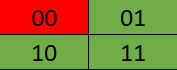
\includegraphics[width=67mm, keepaspectratio]{figures/sirf_sil1.png}\hspace{1cm}
	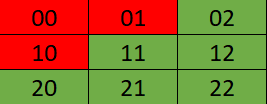
\includegraphics[width=67mm, keepaspectratio]{figures/sirf_sil2.png}\\\vspace{1cm}
	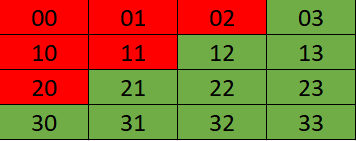
\includegraphics[width=67mm, keepaspectratio]{figures/sirf_sil3.png}\hspace{1cm}
	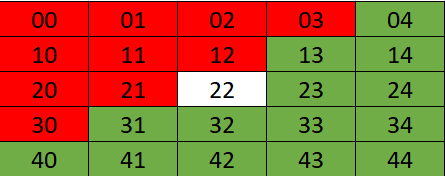
\includegraphics[width=67mm, keepaspectratio]{figures/sirf_sil4.png}
	\caption{Megengedett kombinációk az integritás szinteknek megfelelően, sorrendben SIL1, SIL2, SIL3, SIL4 \emph{Forrás}: SIRF 400}
	\label{fig:sirfSIL}
\end{figure}
\section{Top-down módszerek}
\subsection{Funkcionális analízis}
A funkcionális analízis (FA) egy alapvető módszer a rendszer kritikus funkciói megértéséhez és tervezéséhez.
Az FA elvégzése nélkülözhetetlen a RAMS menedzsmentben és a rendszertervezésben.
A vizsgálat célja, hogy információt adjon arról, ami befolyásolja a rendszer funkcióit és alapot nyújtson a RAMS menedzsmenthez.

Az FA még a specifikáció, modellezés, szimuláció, validáció és verifikáció lépéseinél is alkalmazható.
Ezért a funkcionális analízis gyakran fontos módszerként alkalmazzák a rendszer funkcionális struktúrájának meghatározására.
A funkcionális analízist általában az alábbi két megközelítésben alkalmazzák:
\begin{itemize}
    \item Struktúrált Analízis és Design módszer (SADT\footnote{Structured Analysis and Design Technique})
    \item Funkcionális Analízis Rendszer módszer (FAST\footnote{Functional Analysis System Technique})
\end{itemize}
SADT-ot több iparágban is alkalmazzák. 
Ez egy diagramszerű koncepció, mely segítségével megérthető és leírhatók a rendszer funkcionális viselkedési és interfészei.
A módszer számos elemet szolgáltat az aktivitások és adatfolyamok reprezentálására és nyilakat ezek kapcsolataihoz, ahhogy az alábbi \ref{fig:sadt} ábrán látható, ami egy példa az SADT-ra.

\begin{figure}
    \footnotesize
    \centering
    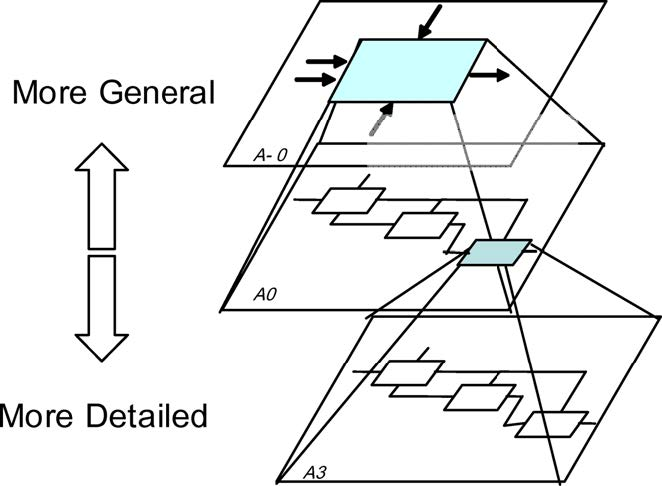
\includegraphics[width=100mm, keepaspectratio]{figures/roh2007.jpg}
    \caption{SADT modell (Forrás: Roh, 2007\cite{doi:10.1080/13675560701478240})}
    \label{fig:sadt}
\end{figure}

A FAST Charles Bytheway fejlesztette ki 1964-ben. Ezt a módszert is sok iparág használja.
A FAST-ot azokban a szituációkban lehetséges felhasználni, ahol a funkciókat logikai sorozatban lehet ábrázoloni, ezáltal priorizálni őket és megvizsgálni a függőségeit.
Ez a módszer nem alkalmas funkcionális problémák megoldására, inkább feltárni a rendszer alapvető funkcionális karakterisztikáit.
Az \ref{fig:fast} ábra egy példa a FAST modellre Kaufmann (1982) által.

\begin{figure}
    \footnotesize
    \centering
    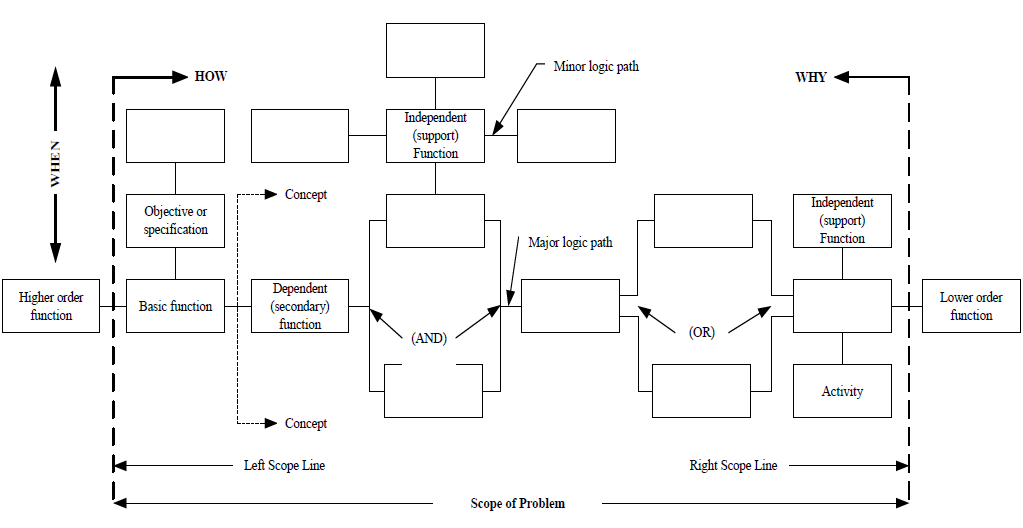
\includegraphics[width=150mm, keepaspectratio]{figures/fast.png}
    \caption{FAST modell (Forrás: Kaufmann, 1982, \cite{Kaufmann:1982})}
    \label{fig:fast}
\end{figure}

\subsection{Hibafa analízis}
A Hibafa analízis (FTA\footnote{Fault Tree Analysis}) egy szisztematikus, deduktív és logaikai módszer a rendszerhiba (Top event) okainak feltárására, modellezésére, vizsgálatára.
Az FTA-t lehet az egyek legmegbízhatóbb eszköznek tekinteni a hiba eset logaikai kiértékelésében biztonsági és megbízhatósági szempontból. \cite{Ericson}

A hibafát H. Watson és Allison B. Mearns fejlesztette ki 1962-ben, akik együtt dolgoztak a US Bell Company laboratóriumában. Később a Boeing Company is elkezdte használni a módszert, hogy meghatározza a biztonsági faktorokat, melyek fegyverrendszerekre lehetnek hatással.
Az 1960-as években a kereskedelmi repülés, '70-es években a nukleáris energiaipar, '80-as években a vegyipar, '90-es években közlekedési ipar is elkezdte használni a módszert biztonságosság és megbízhatóság felmérésére (Ericson, 1999).

Az analízis az előfordulható hibamódok egy részhalmazára fokuszál, különös tekintettel azokra, amik katasztrofális hibát okozhatnak.
A kapuk (gate), események (event) és vágások (cut set) jelentik a legfőbb elemzési pontjait.
A logikai diagramm - 'ÉS' és 'VAGY' kapuk - adja meg a FTA eredményét.
A hibaesetek adják meg a kapuk bemeneteit és a vágások adják meg azoknak a hibaeseteknek halmazát, ami rendszerhibát okozhat.
Az FTA-t szokás az FMECA\footnote{Failure Mode Effect and Criticallity Analysis}-val, Markov analízissel és ETA\footnote{Event Tree analysis}-val együttesen használni, hogy elfedjék az FTA limitációit (Stapelberg, 2008; BE EN 60812, 2006).

\begin{figure}
    \footnotesize
    \centering
    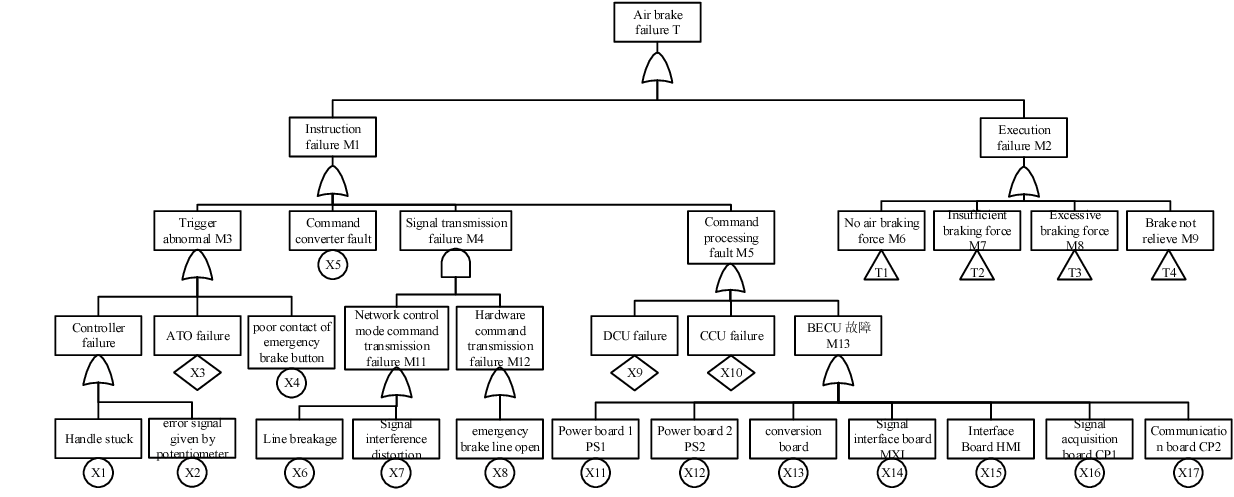
\includegraphics[width=150mm, keepaspectratio]{figures/fta1.png}
    \caption{Egy hibafa példa pneumatikus fékrendszer meghibásodásához (Forrás: Long, 2017 \cite{Long2017BrakingSM})}
\end{figure}

\subsection{Megbízhatósági blokkdiagram analízis}
A Megbízhatósági blokkdiagram (RBD\footnote{Reliability Block Diagram}) egy vizuális elemzési módszer aminek segítségével könnyen reprezentálható a rendszer logikailag összekötött struktúrája.
Az RBD blokkjai ábrázolják a rendszer eredményes működését. Az elemzés különböző szinten jelentkezhet, mind kvalitatív, mind kvantitatív formában (BS EN 61078, 2006; BS EN 60300-3-1, 2004).

A diagramm felépíthető egyenesen a rendszer funkciónális modelljéből, ami szisztematikusan megjeleníti a funkcionális utakat.
Sok különböző rendszerkonfigurációt képes kifejezni, például, soros, párhuzamos, rendundáns, ,,standby'' stb., ahogy az az \ref{fig:rdb} ábrán is látszik.
Az RBD-t általában abban az esetben használják, amikor különböző változatait és komprumisszumait kell értékelni megbízhatósági és elérhetőségi szempontból.
\begin{figure}
    \footnotesize
    \centering
    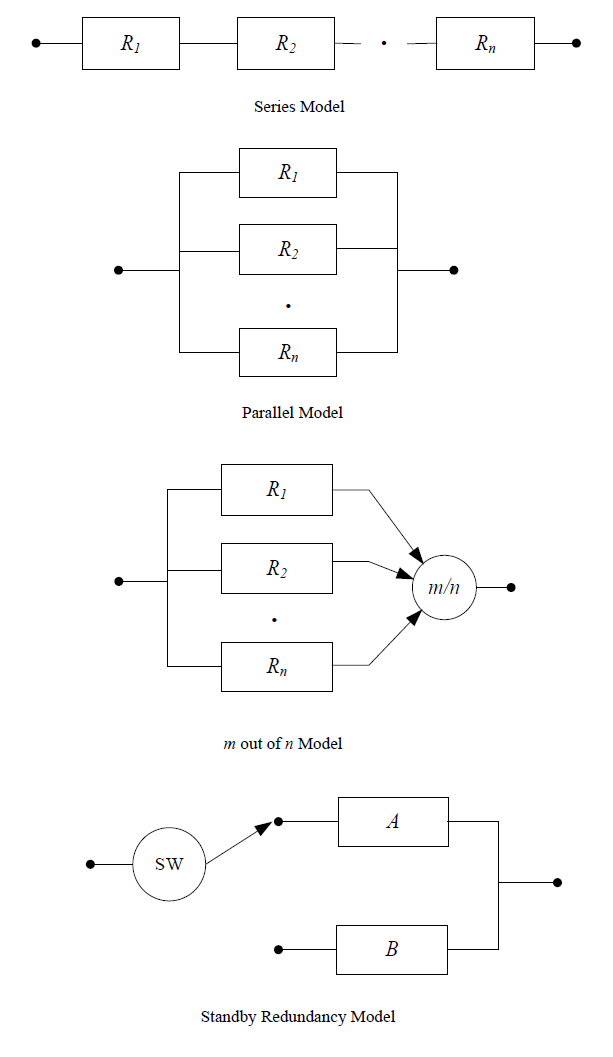
\includegraphics[width=80mm, keepaspectratio]{figures/rbd1.png}
    \caption{Különböző RDB modellek (Forrás: BS EN 61078, 2006)}
    \label{fig:rdb}
\end{figure}

\subsection{Közös hibaforrás azonosítás}

\section{Bottom-up módszerek}
\subsection{FMEA analízis}
Az Hibamód és hatás analízis (FMEA\footnote{Failure Mode and Effect Analysis}) egy biztonságossági és megbízhatősági kiértékelő módszer, ami képes felmérni a rendszer összem komponensének összes potenciális hibamódját, ami kihathat az egész rendszer teljesítményére.
A módszer továbbá azonosítja azokat a módszereket is, amikkel elkerülhetők a hibamódok és hogyan lehetséges csökkenteni azok hatását.

A módszert eredetileg FMECA\footnote{Failure Mode Effect and Criticality Analysis} néven említették, amiben a ,C' betű a hibamód kritikusságát jellemezte.
Bár a két módszert gyakran szinonímaként használják, teljesen más a megközelítésük.
Általában az FMEA-t a hibamód hatásának súlyosságát minősíti, míg az FMECA a hibamód frekvenciáját is megvizsgálja a súlyosság mellett.
A súlyosság és a frekvencia kombinációját a rendszer kritikusságnak vagy kockázatának nevezik (MIL-STD-1629A, 1980).

A módszer során minimum a következő nyolc információt kell megállapítani:
\begin{enumerate}
    \item Hibamódok (Failure mode)
    \item A hibamód hatása a rendszerre
    \item A hibamód miatt bekövetkezett rendszerszintű hiba
    \item A veszélyek baleseti hatása
    \item A hibamód és/vagy veszély okozati tényezőit
    \item Hogyan lehet a hibamódot detektálni
    \item Javaslatok
    \item A felderített veszély kockázatát
\end{enumerate}

A módszert több szempontból is el lehet végezni.
Ez lehetnek Funkcionális megközelítés, Struktúrális megközelítés és a ,,hibrid'' megoldás.
Az első megközelítésben a funkciók céljának lehetséges hibás működését veszi figyelembe.
Ez a módszer alkalmazható szoftverek esetében is.

A második megközelítés leginkább hardver elemeken végzett lehetséges hibamódokra öszpontosít.
A ,,hibrid'' megközelítés először a funkcionális analízissel kezdődik, aminek fókusza átvált a hardverre (Ericson, 2005).

Lehetséges példák a funkcionális hibamódokra:
\begin{itemize}
    \item A funkció nem működik
    \item A funkció nem megfelelően működik
    \item A funkció idő előtt hajtódik végre
    \item A funkció hibás vagy félrevezető információt szolgáltat
    \item A funkció nem hibásodik meg biztonságosan
\end{itemize}
Lehetséges hardver hibamód kategóriák:
\begin{itemize}
    \item Teljes meghibásodás
    \item Részleges meghibásodás (például: tolerancián kívül)
    \item Időszakos meghibásodás
\end{itemize}
Lehetséges hardver hibamódok:
\begin{itemize}
    \item Szakadás
    \item Rövidzárlat
    \item Tolerancián kívül
    \item Szivárgás
    \item Meleg felület
    \item Elhajlás
    \item Túl/alulméretezett
    \item Megrepedt
    \item Rideg
    \item Elmozdult
    \item Korrodált
    \item stb.
\end{itemize}
Lehetséges hibamódok szoftvereknél:
\begin{itemize}
    \item A szoftver funkció meghibásodik
    \item A funkció hibás eredményt szolgáltat
    \item A funkció idő előtt meghívódik
    \item Elküldetlen üzenetek
    \item Túl korán/későn küldött üzenet
    \item Hibás üzenet
    \item Megáll vagy összeomlik a szoftver
    \item Belső kapacitásoknál többet igényel a szoftver
    \item Szoftver ,,startup'' hiba
    \item Lassú válaszidő
\end{itemize}

\subsection{HAZOP analízis}

\subsection{LOPA}
Layer of Protection Analysis (LOPA) \cite{LOPA1}